\section{Results and Analysis}
\subsection{Simulation Methodology}
The key problem that we address is the mitigation of power consumption attacks on individual sensor nodes in Wireless Sensor Networks.  One central issue underlies the surface details of all wireless sensor nodes: A limited power supply. The nature of wireless sensor networks is such that it is likely optimal to draw power remotely, from a source such as a battery. The battery would also have to be quite small so it would not impede the actual duties of the node and take up space making the manufacturing process more costly, and less effective. 

We turned immediately to analyze the source from which the power was being drawn. Using a piece of software called NS3, we simulated the time required by the attacker to compromise a wireless radio by sending packets at a rate of 1/10 ms. The wireless radios were equipped with batteries that contained a certain internal acid. The acids tested are seen in the table in the next section. The weight of each battery was varied from 0.1 mg to 1 mg and 660 simulation results were collected. 

Next, to gain a more thorough understanding of the implications of different kinds of power consumption attacks that are performed on WSNs we created a simulation environment in python, in which the user could define: the packet size (in bits), the initial energy in each node (in Joules), the power required to transmit packets (in Watts), the power required to receive packets (in watts), the speed of the transmission radios (in bits per second). 

As stated in the introduction we specifically examined two specific kinds of attacks, the standard denial of sleep attack and the routing attack. Below are diagrams of each attack for the reader to have a clear image of what was simulated, and for the sake of completeness one attack that was not simulated.

\begin{figure}[H]
\caption{Standard Denial-of-Sleep Attack}
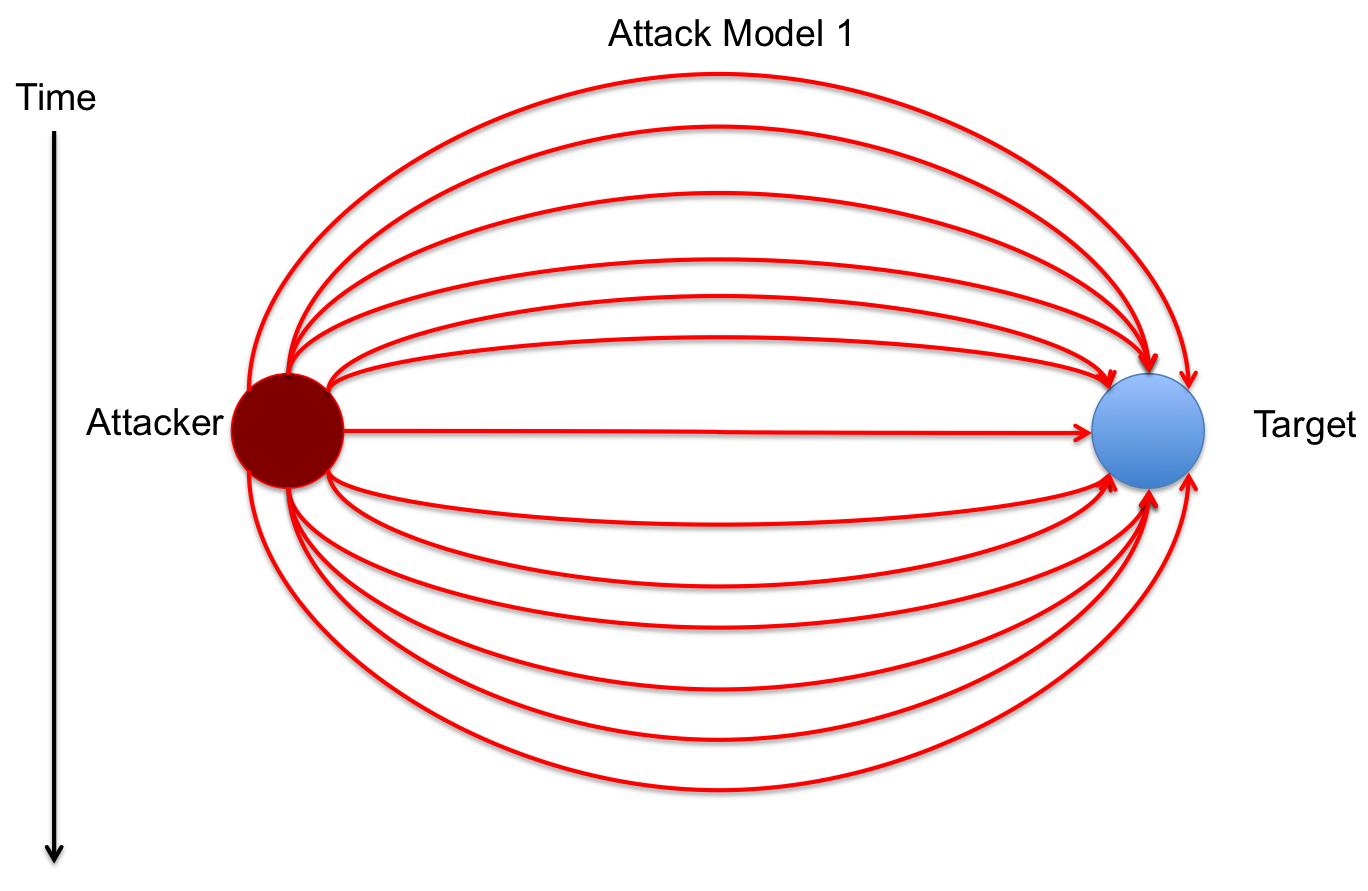
\includegraphics[width = \linewidth]{Figures/AModel1.png}
\end{figure}

The image above depicts the ``standard denial-of-sleep attack" the attacker continuously sends packets to the target to keep it in the ``awake" mode so that power is drawn from the battery more quickly.

\begin{figure}[H]
\caption{Inverse Denial-of-Sleep Attack}
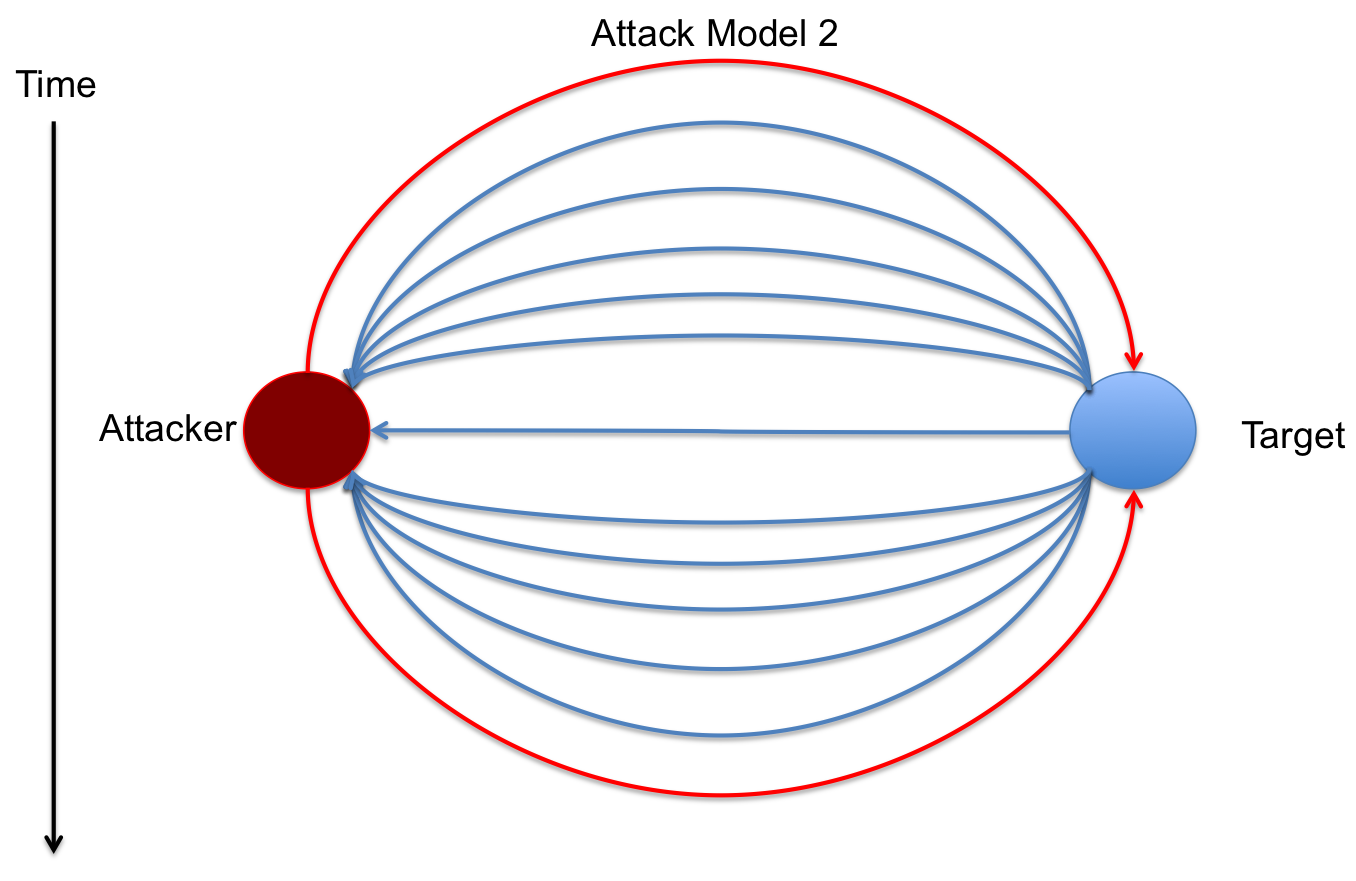
\includegraphics[width = \linewidth]{Figures/AModel2.png}
\end{figure}

The image above depicts the ``inverse denial-of-sleep attack" the attacker sends a request to the target to force it to transmit over and over again, this image represents a system where an acknowledgement is required after a transmission, but is never sent by the attacker we defer simulation of this form of attack to future work.

\begin{figure}[H]
\caption{Routing Power Draw Attack}
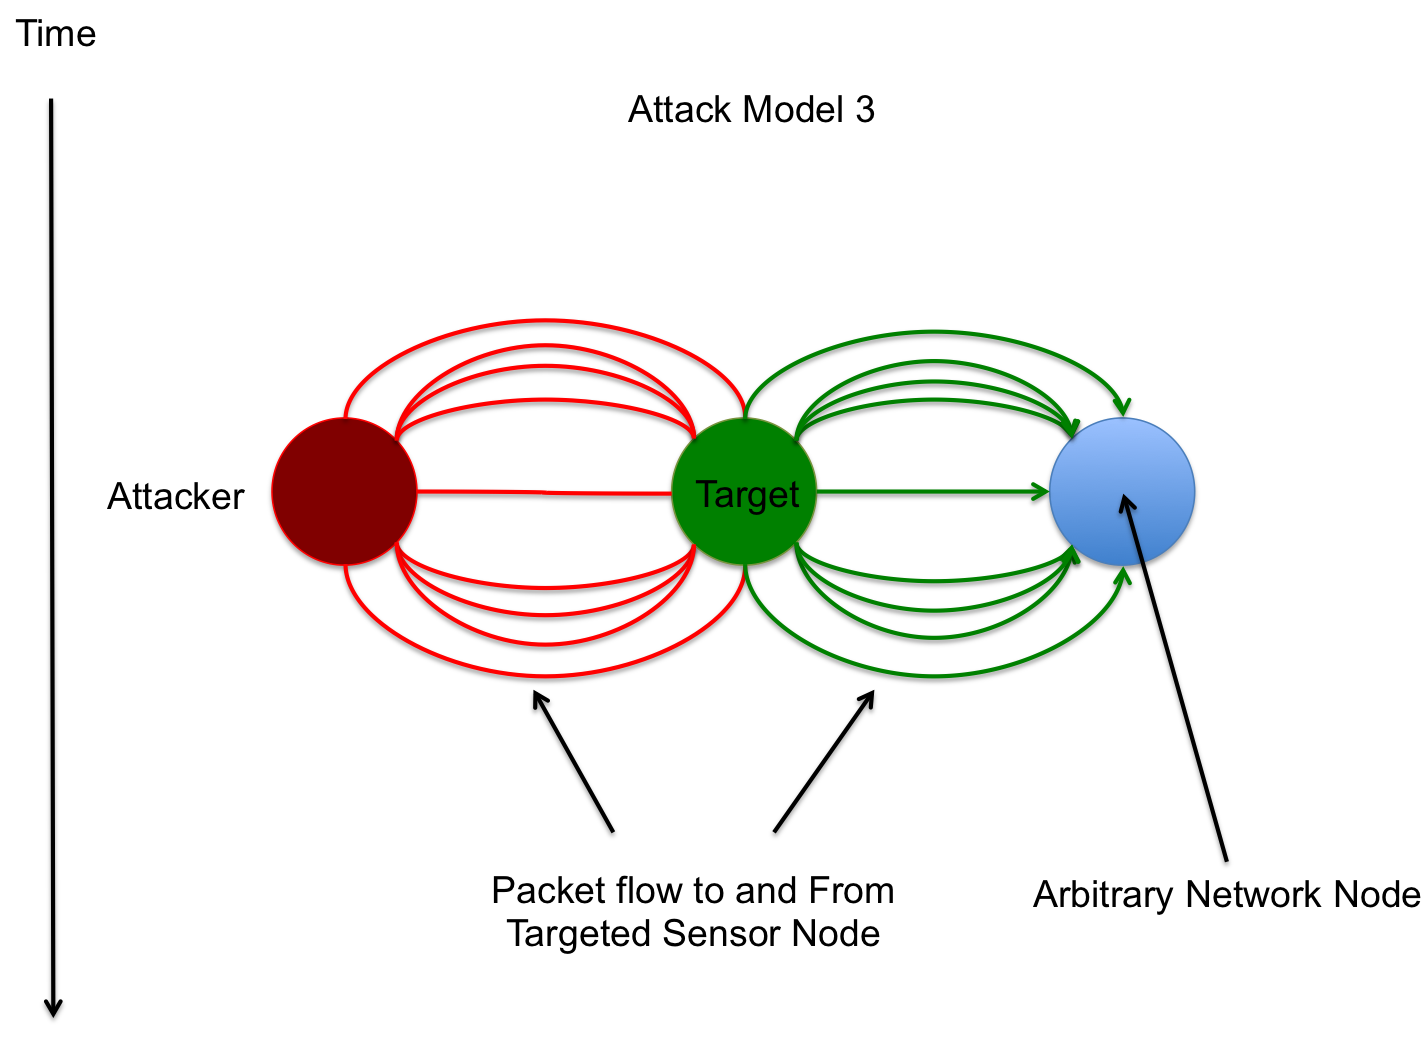
\includegraphics[width = \linewidth]{Figures/AModel3.png}
\end{figure}

The image above depicts the ``routing power draw attack" the attacker routes through the target node which causes the target to go through both transmitting and receiving procedures, it is a particularly vicious attack.
\subsection{Simulation Results}

The first results came from running the standard denial of sleep attack on various different battery types, the size of transmitted packets varied in powers of two from the size of two bits to one kilo bit, and the packet transmission rate was constant at one packet every ten milliseconds.

\begin{figure}[H]
\caption{Battery Compromise Table} 
		\begin{tabular}{| l | c | c | r |}
			\hline
			\textbf{B-Type} & \textbf{TTC(Min)}& \textbf{MTTC} & \textbf{TTC(Max)} \\
			\hline
			\hline
			\textcolor{red}{Lead Acid} & 0.2789 s & 9.8798 s & 27.0307 s \\
			\hline
			\textcolor{blue}{Alkaline Long Life} & 0.7589 s & 27.1017 s & 74.1107 s \\
			\hline
			\textcolor{red}{Carbon-Zinc} &  0.2489 s & 8.7950 s & 24.0700 s \\
			\hline
			\textcolor{blue}{NiMH} & 0.6489 s & 23.0336 s & 62.9907 s \\
			\hline
			\textcolor{red}{Nickle-Cadmium} & 0.2689 s & 9.4734 s & 25.9207 s \\
			\hline
			\textcolor{blue}{Lithium-Ion} & 0.8689 s & 31.1701 s & 85.2400 s \\
			\hline
		\end{tabular}
\end{figure}

In the table above ``B-type" represents the type of acid that was tested, ``TTC" represents the Time to Compromise (the time it takes to deplete all the energy from the sensor node), ``MTTC" is the mean time to compromise. The batteries that are highlighted in blue showed a marginally better resistance to the standard denial-of-sleep attack, while those in red were compromised far too quickly to be implemented and deployed as effective defenses. As the table plainly shows the Lithium-Ion battery was the most resistant to the standard denial-of-sleep attack. Below we show how the change in packet size affected the time to compromise of the Lithium-Ion battery to see how weight affects the time to compromise. 

\begin{figure}[H]
\caption{Time to Compromise for Battery Weights}
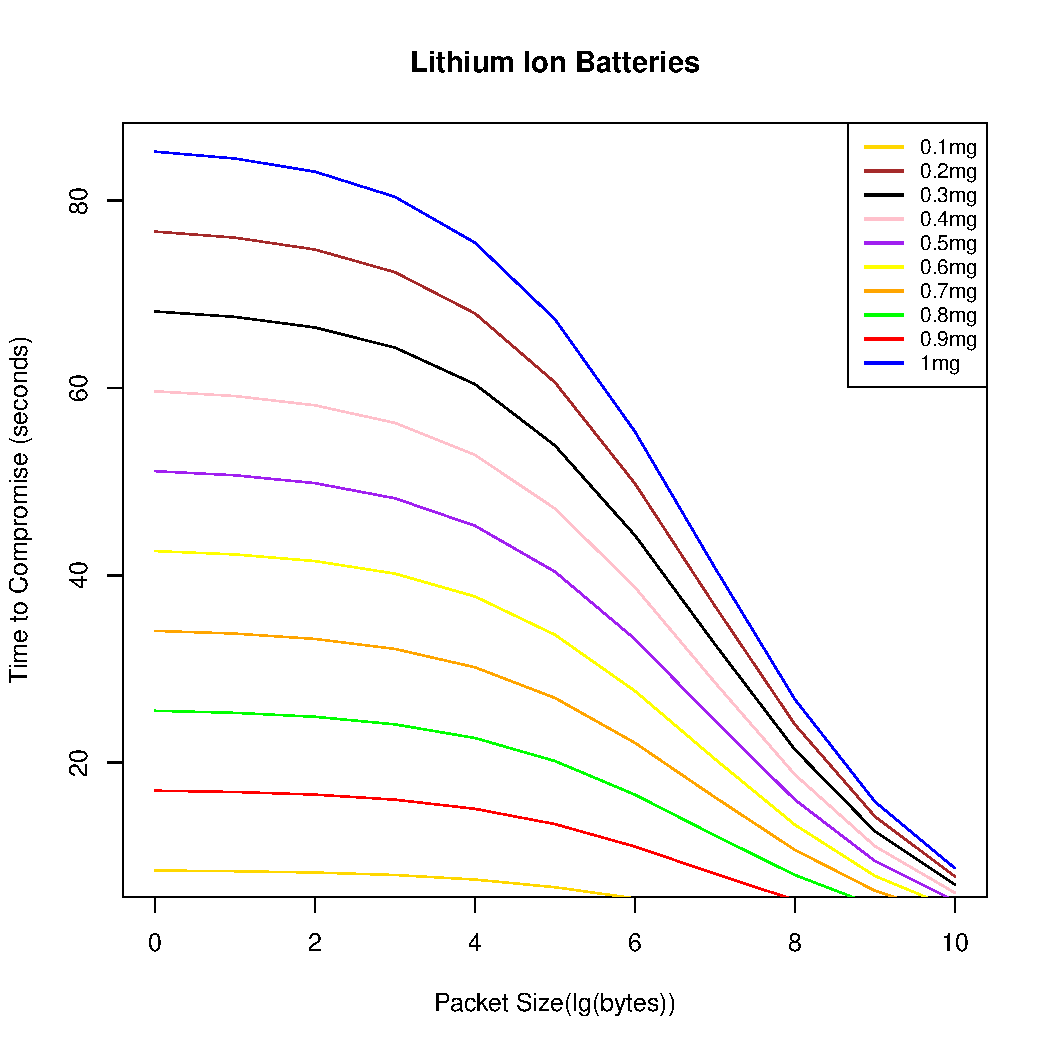
\includegraphics[ width=\linewidth]{Figures/LINBATTTC.pdf}
\end{figure}

Probably the biggest take away from this graph is the fact that all battery weights seem to converge in terms of time to compromise as the packet size being transmitted increases. From this graph we can tell that it would be more effective to use higher battery weights only when the packet sizes are kept relatively small. However, if the packet size is sufficiently large then it would be in the best interest of the distributor to choose a smaller weight. 

In our second simulation we tested the time to compromise a sensor node for two of the previously discussed attack, the standard denial-of-sleep attack and as well as the routing power draw attack. The table below shows some of the preliminary results from the second simulation. 



